\documentclass[12pt]{article} % use larger type; default would be 10pt
\usepackage[utf8]{inputenc} % set input encoding (not needed with XeLaTeX)

%%% PAGE DIMENSIONS
\usepackage{geometry} % to change the page dimensions
\geometry{letterpaper} % or letterpaper (US) or a5paper or....
 \geometry{margin=1in} % for example, change the margins to 2 inches all round
% \geometry{landscape} % set up the page for landscape
%   read geometry.pdf for detailed page layout information

%%% PACKAGES
\usepackage{graphicx} % support the \includegraphics command and options
\usepackage{setspace}
\doublespacing
\usepackage[parfill]{parskip} % Activate to begin paragraphs with an empty line rather than an indent
\usepackage{booktabs} % for much better looking tables
\usepackage{array} % for better arrays (eg matrices) in maths
\usepackage{paralist} % very flexible & customisable lists (eg. enumerate/itemize, etc.)
\usepackage{verbatim} % adds environment for commenting out blocks of text & for better verbatim
\usepackage{subfig} % make it possible to include more than one captioned figure/table in a single float
% These packages are all incorporated in the memoir class to one degree or another...
\usepackage{amsmath} %Allow math
\usepackage{appendix} %Allow for creation of appendicies

%Allow big first letter in Paragraph
\usepackage{type1cm}
\usepackage{lettrine}

%DEFINE VARIABLES
\newcommand{\classnumber}{AAE\:412\:-\:Team\:32:}
\newcommand{\reportnumber}{Final Project}
\newcommand{\TAname}{Dr. Gregory Blaisdell}

%%% HEADERS & FOOTERS
\usepackage{fancyhdr} % This should be set AFTER setting up the page geometry
\pagestyle{fancy} % options: empty , plain , fancy
\renewcommand{\headrulewidth}{0pt} % customise the layout...
\lhead{}\chead{}\rhead{}
\lfoot{}\cfoot{\thepage\\Purdue University}\rfoot{}

%%% SECTION TITLE APPEARANCE
\usepackage{sectsty}
\allsectionsfont{\fontsize{12}{15}\centering\textbf} % (See the fntguide.pdf for font help)
\renewcommand{\thesection}{\Roman{section}.} 
\renewcommand{\thesubsection}{\textbf{\Alph{subsection}.}}
% (This matches ConTeXt defaults)
\usepackage[font=small,labelfont=bf]{caption} % Required for specifying captions to tables and figures

\renewcommand{\appendixname}{APPENDIX} %Change  Appendix Title to spell out the word

%%% END Article customizations

%%%MATLAB CODE
\usepackage[numbered,framed]{matlab-prettifier}
\renewcommand*{\lstlistlistingname}{List of MATLAB Code Snippets} %Change MATLAB ToC Title


%%% The "real" document content comes below...

\title{\classnumber\:\reportnumber}
\author{Jay Blake\\Devin Eubanks\\Brad Lock\\Purdue University}

\begin{document}
\maketitle
\vspace{2in}
\begin{center}
    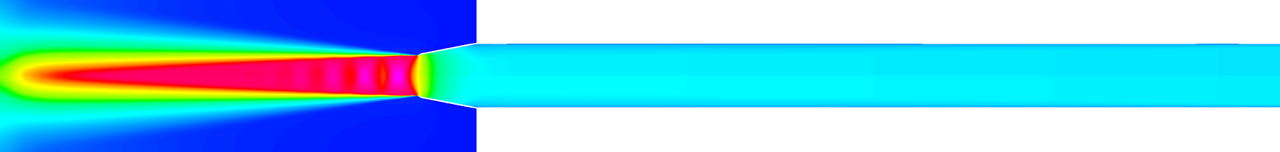
\includegraphics[width=\linewidth]{CoverPicture.png}
\end{center}
\clearpage
\begin{center}
{\Large\textbf{\classnumber\:\reportnumber}}\\
\vspace*{24pt}
Jay Blake\footnote{Engineer, School of Aeronautics and Astronautics, 701 W Stadium Ave, West Lafayette, IN 47907}, Devin M. Eubanks\footnote{Engineer, School of Aeronautics and Astronautics, 701 W Stadium Ave, West Lafayette, IN 47907}, and Bradley W. Lock\footnote{Engineer, School of Aeronautics and Astronautics, 701 W Stadium Ave, West Lafayette, IN 47907}\\
\textit{Purdue University, West Lafayette, IN, 47907}
\end{center}
\vspace*{48pt}
\textbf{\hspace{36pt}[Abstract] A Computational Fluid Dynamics simulation was ran on three nozzle geometries, defined by M. T.. Trumper, P. Behrouzi, and J. J. Mcguirk in \textit{Influence  of  nozzle  exit  conditions on  the  near-field  development  of  high  subsonic  and  underexpanded  axisymmetric  jets}. Analysis was performed on boundary layer and jet plume properties for supersonic conditions using a Nozzle Pressure Ratio of 2.2. An additional analysis was performed on one of the nozzles to determine flow properties of jet exhaust rather than air.}
\vspace*{36pt}
\section*{Nomenclature}
\begin{table}[ht]
    %\centering
    \begin{tabular}{l c l}
       $\alpha$&=&Angle of Attack\\
       CFD&=&Computational Fluid Dynamics\\
         M&=&Mach Number\\
         NPR&=&Nozzle Pressure Ratio\\
         $p$&=&Pressure\\
         $p_0$&=&Stagnation Pressure\\
         V&=&Velocity
    \end{tabular}
    \label{tab:nomenclature}
\end{table}

\section{Introduction}
\lettrine{T}{he} purpose of this project is to perform a Computational Fluid Dynamics (CFD) analysis of the geometries provided in the paper by M. T. Trumper, et al. \cite{MilesT.Trumper2018IoNE} These geometries are listed in Figure \ref{fig:og_geometry}. The goal of the project is to perform measurements of the inlet and outlet boundary layers, to understand the properties of the jet near field, and to compare the calculated results with those of Trumper, et al.

\begin{figure}[ht]
    \centering
    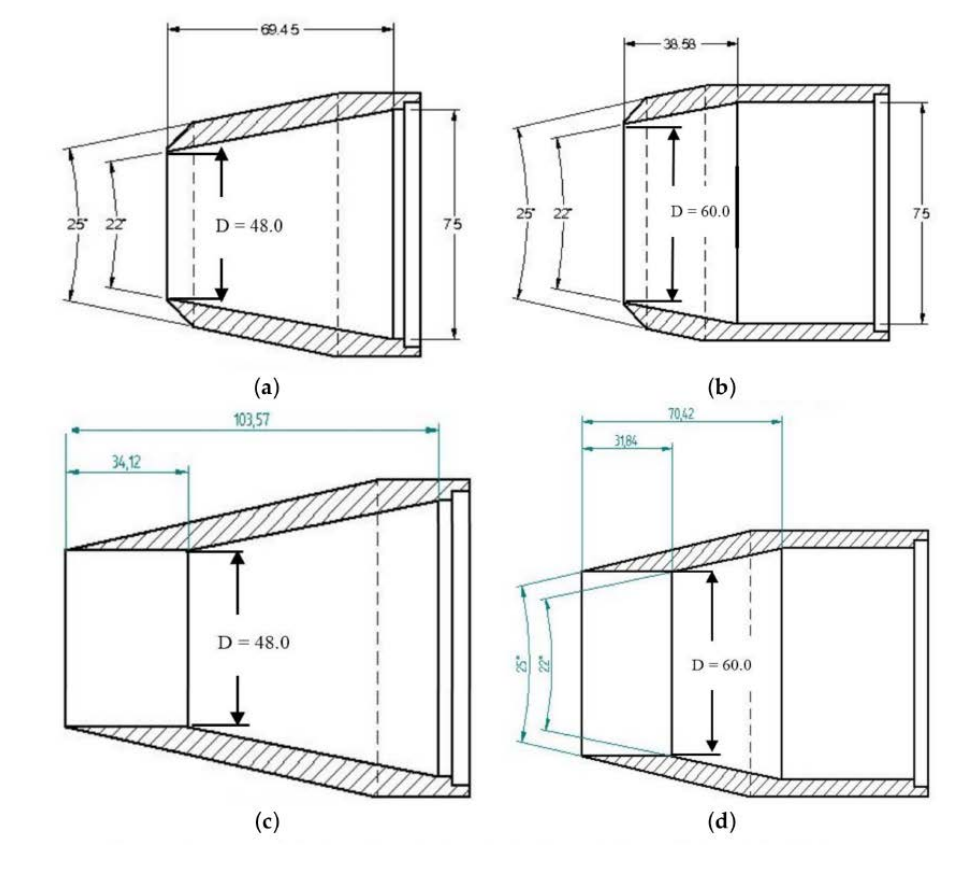
\includegraphics[width = 4in]{OG_Geometry.PNG}
    \caption{Provided Geometries}
    \label{fig:og_geometry}
\end{figure}

\section{Numerical Solution}
\subsection{Geometry}
ANSYS Fluent was used to develop a numerical solution for Nozzles (a), (b), and (c) shown in Figure \ref{fig:og_geometry}. For each nozzle, Design Modeler was used to create the geometry. In the paper written by Trumper, et al., it was noted that the first 10-15 exit diameters around the output of a jet are important in the analysis of jet plumes \cite{MilesT.Trumper2018IoNE}, so the outer domain was defined out to 20 exit diameters for each case. The inlet pipe length was chosen such that the boundary layer at the nozzle inlet was 29mm, matching the boundary layer defined in the paper. The domains used are shown with meshing in Section \ref{section:mesh}.\par

In order to determine the pipe length required to reach the proper boundary layer, the pipe was extended to 2 meters and ran in Fluent using the boundary conditions in Table \ref{tab:boundary}. Then, CFD Post was used to show the Mach contours and the location within the pipe was found visually to be 1.21 meters from the inlet, as shown in Figure \ref{fig:boundarylength}. The pipe was then shortened to this length in all geometries.

\begin{figure}[ht]
    \centering
    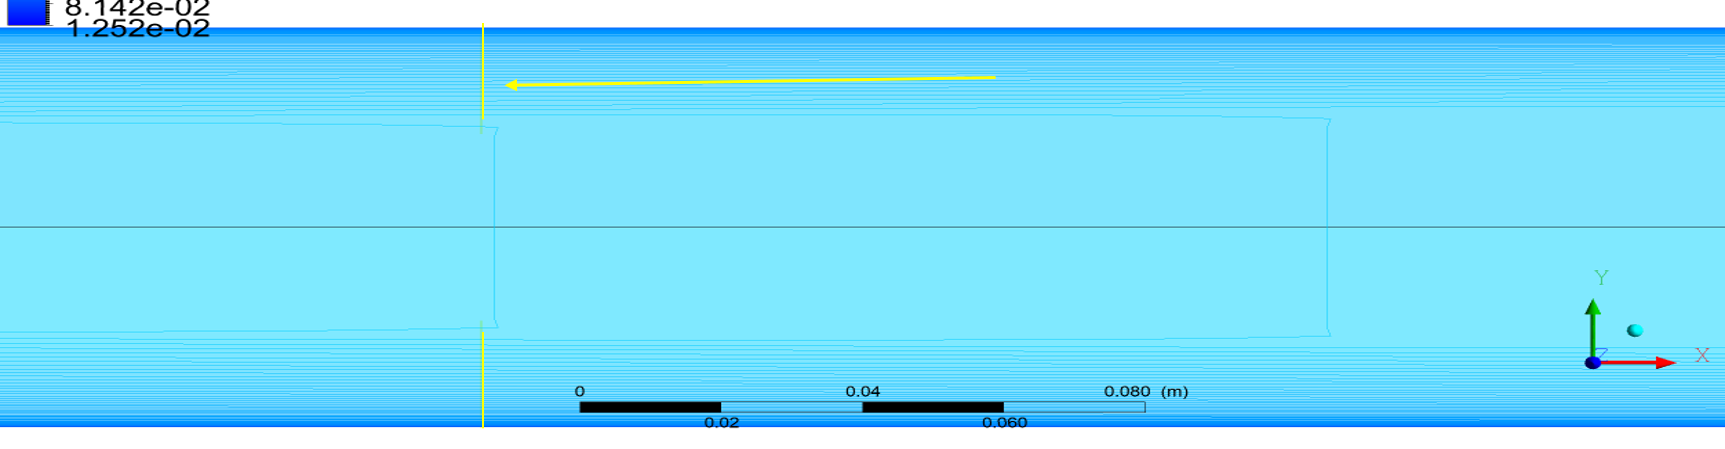
\includegraphics[width = \linewidth]{BoundaryLength.PNG}
    \caption{CFD Post - Pipe Length}
    \label{fig:boundarylength}
\end{figure}

\subsection{Meshing}\label{section:mesh}
Insert information here about meshing. To refer to meshes, use Figure \ref{fig:geomA}, \ref{fig:geomB}, and \ref{fig:geomC} for (a), (b), and (c) respectively.

\begin{figure}[ht]
    \centering
    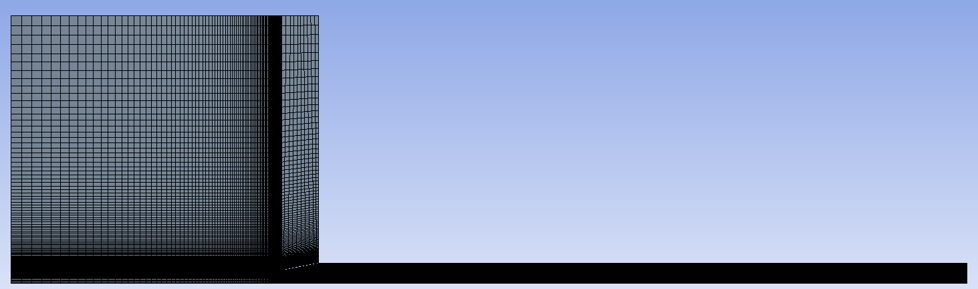
\includegraphics[width = \linewidth]{NozzleA_Mesh.PNG}
    \caption{Nozzle (a) Mesh}
    \label{fig:geomA}
\end{figure}

%\begin{figure}[ht]
%    \centering
%    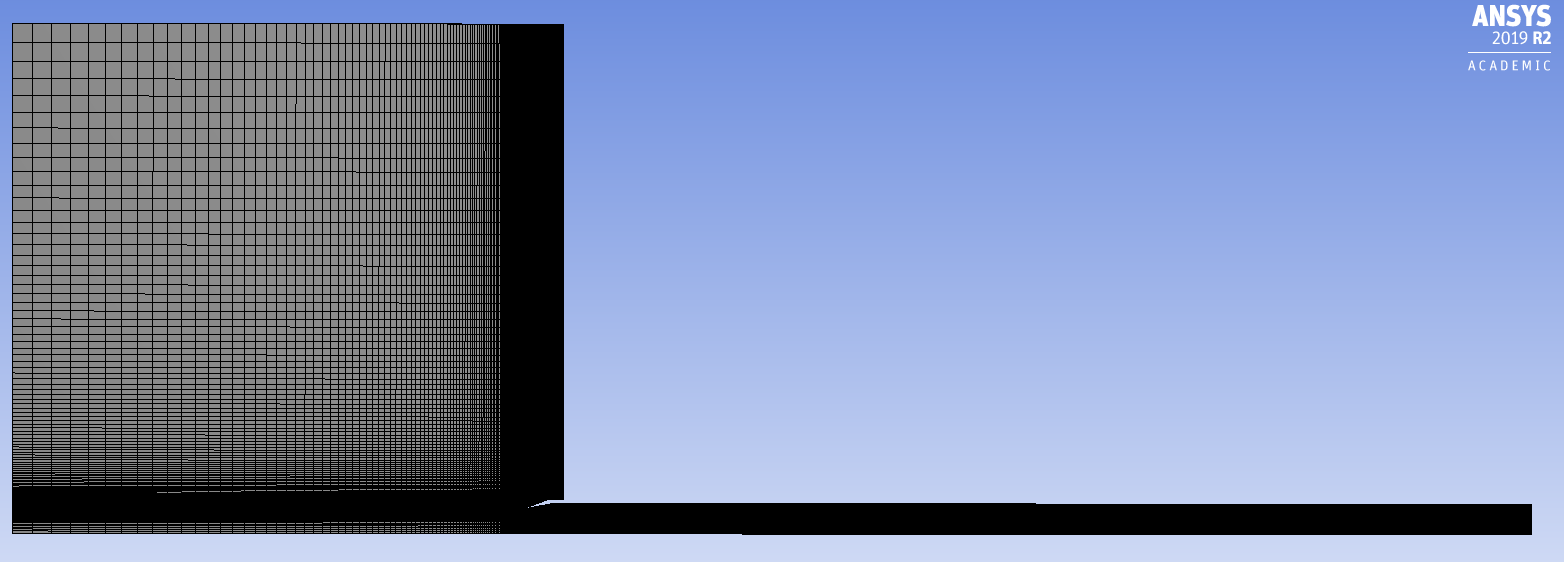
\includegraphics[width = 4in]{NozzleB_Mesh.PNG}
%    \caption{Nozzle (b) Mesh}
%    \label{fig:geomB}
%\end{figure}

%\begin{figure}[ht]
%    \centering
%    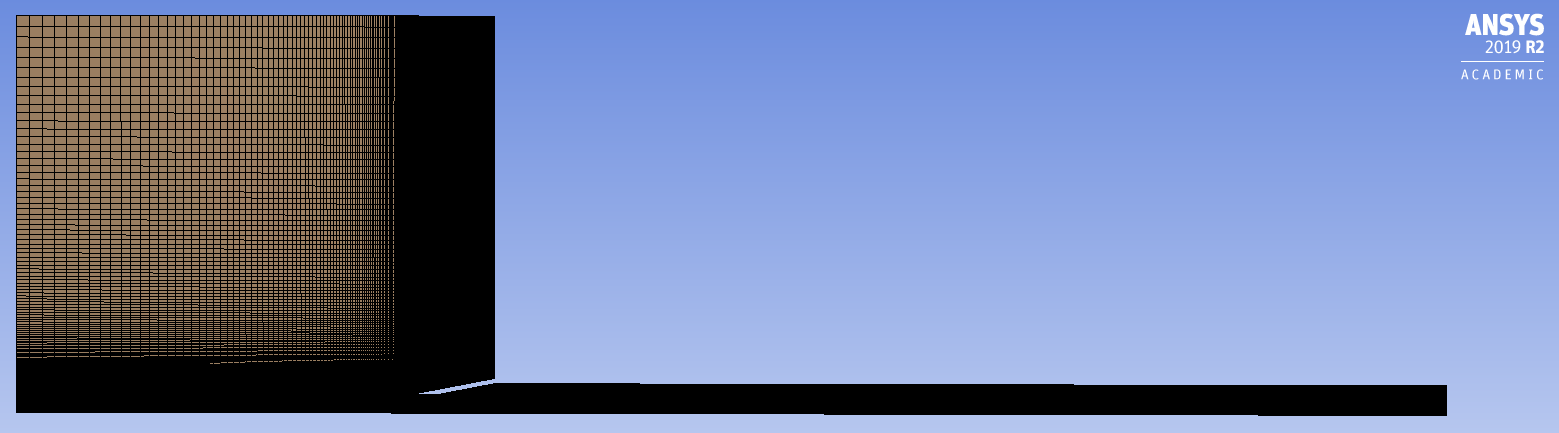
\includegraphics[width = 4in]{NozzleC_Mesh.PNG}
%    \caption{Nozzle (c) Mesh}
%    \label{fig:geomC}
%\end{figure}

A grid comparison was completed on Nozzle A to ensure the aspect ratio was maintained between the coarse and fine grids. A close-up view of these grids is shown in Figure \ref{fig:gridcompareA}. The aspect ratio for the coarse grid was 252.81; the aspect ratio for the fine grid was 251.72.

\begin{figure}[ht]
    \centering
    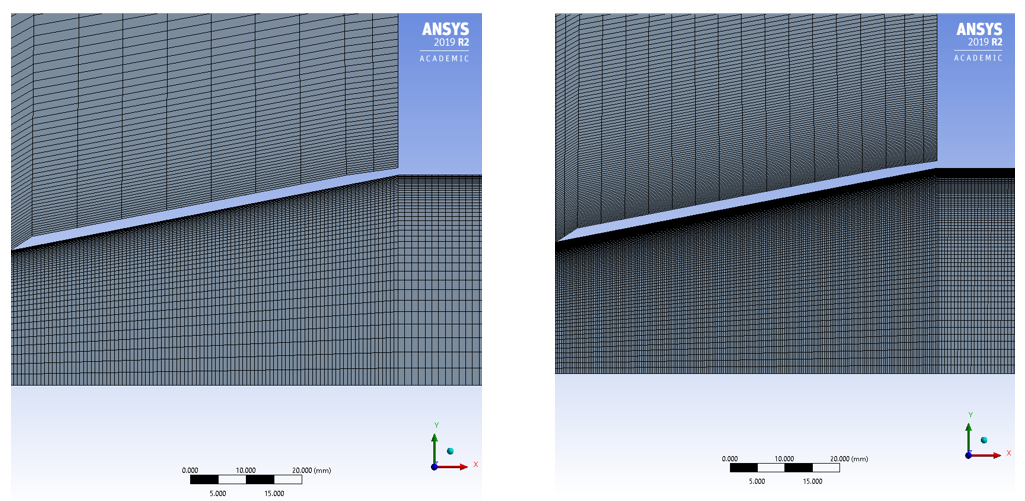
\includegraphics[width = \linewidth]{GridCompareA.png}
    \caption{Nozzle (a) Grid Comparison}
    \label{fig:gridcompareA}
\end{figure}

\subsection{Fluent}\label{section:fluent}
The following boundary conditions were used for each geometry, shown in Table \ref{tab:boundary}

\begin{table}[ht]
    \caption{Boundary Conditions}
    \centering
    \begin{tabular}{l|l}
        Named Selection&Boundary Condition\\
        \hline
        nozzle-wall&wall\\
        farfield&pressure-farfield\\
        nozzle-inlet&pressure-inlet\\
        ambient-inlet&velocity-inlet\\
        axis&axis\\
        \hline
    \end{tabular}
    \label{tab:boundary}
\end{table}

For fine and course grids with each geometry, the parameters used in Fluent are shown in Tables \ref{tab:parameter1} and \ref{tab:parameter2}. 

\begin{table}[ht]
    \caption{Fluent Parameters}
    \centering
    \begin{tabular}{l|l}
        \multicolumn{2}{c}{Physics Parameters}\\
        \hline
        Energy&On\\
        Viscosity&Realizable k-$\epsilon$\\
        \hline
        \multicolumn{2}{c}{}\\
        \multicolumn{2}{c}{Controls}\\
        \hline
        Type&Explicit\\
        Flow&2\textsuperscript{nd} Order Upwind\\
        \hline
    \end{tabular}
    \label{tab:parameter1}
\end{table}

\begin{table}[ht]
    \caption{Boundary Condition Parameters}
    \centering
    \begin{tabular}{l|l|l}
        \multicolumn{3}{c}{Nozzle Inlet}\\
        Parameter&Value&Unit\\
        \hline
        $p_0$&121590&Pa\\
        \hline
        \multicolumn{3}{c}{}\\
        \multicolumn{3}{c}{Ambient Inlet}\\
        Parameter&Value&Unit\\
        \hline
        $V_{axial}$&-10&m/s\\
        \hline
        \multicolumn{3}{c}{}\\
        \multicolumn{3}{c}{Far Field}\\
        Parameter&Value&Unit\\
        \hline
        $p$&20&Pa\\
        $M$&.1&\\
        Axial Direction&-1&\\
        \hline
    \end{tabular}
    \label{tab:parameter2}
\end{table}

\clearpage
\section{Results}
This is where we will write our Results Section.  (includes analysis and discussion)

\section{Conclusions}
This is where we will write our Conclusions Section.  (similar to the abstract, but contains a more detailed summary
of the results you found, lessons learned and suggestions for further study (if
appropriate)).

\section{References}
%Note: Do not change this! References are added in BibTex format in AAE412Bib.bib
This is where we will place the references
\nocite{*}
\begingroup
\renewcommand{\section}[2]{}%Remove Extra Title
\bibliographystyle{abbrv}
\bibliography{AAE412Bib}
\endgroup


\clearpage
{\Large{\color{red}Begin Useful Stuff for learning LaTeX}}

I will attempt to place a graphic in this section with a caption:
\begin{center}
\includegraphics{rootlocus.png}
\captionof{figure}{Sample Root Locus}
\end{center}

\clearpage

\section{Tables}

Coming up in the section below is a table with a caption.

\subsection{Table Subsection}

\begin{table}[ht]
\caption{Sample Table Title} % title of Table
\centering % used for centering table
\begin{tabular}{l | c c c} % a left-text column, vertical line, then 3 centered columns
\hline\hline %inserts double horizontal lines
Heading\#1 & Heading\#2 & Heading\#3 & Heading\#4 \\ [0.5ex] % inserts table
%heading
\hline % inserts single horizontal line
1 & 50 & 837 & 970 \\ % inserting body of the table
2 & 47 & 877 & 230 \\
3 & 31 & 25 & 415 \\
4 & 35 & 144 & 2356 \\
5 & 45 & 300 & 556 \\ [1ex] % [1ex] adds vertical space
\hline %inserts single line
\end{tabular}
\label{table:nonlin} % is used to refer this table in the text
\end{table}

\clearpage

\section{Equations}

This subsection will have equations that are numbered

\subsection{Equations below!}

%Equations with numbering
\begin{align}
1\:+\:k_iL\left(j\omega \right)\:=\:0\\
                          &= 0
\end{align} 

%Equations with no numbering in specific line by using \nonumber
\begin{align}
L\left(s\right)\:=\:\frac{\gamma }{m\left(j\omega \right)^3+c\left(j\omega \right)^2+\gamma \left(j\omega \right)}\nonumber\\
\end{align}

%Equations without numbering
\begin{align*}
j\omega \left(17.24\:-\:7.031\omega^2\right)+\left(1.7235k_i-11.79\omega ^2\right)\:=\:0
\end{align*} 

Of course, math can still be placed using inline text, like this $1.7235k_i\:=\:11.79\omega ^2\:=28.9091$

\clearpage

%Convert to the APPENDIX Portion of the document using the next two lines. 
\appendixpage
\appendix

Appendicies are here

\end{document}
